\section{Evaluation}

To evaluate the effectiveness and potential of \emph{temporal influence analysis} (\tia), we address the following research questions:
\begin{enumerate}[label=\textbf{RQ\arabic*.}, leftmargin=*, align=left]
    \item How does \tia itself perform on real-world Chisel designs in terms of its \emph{fundamental} capabilities, including soundness, precision, and efficiency?
    \item Does \tia have the potential to support \emph{diverse} hardware analysis clients?
    \begin{enumerate}[label=\textbf{RQ2-\arabic*.}, leftmargin=1ex, align=left]
        \item \emph{Hardware Bug Detection.}
        Can \tia support detecting signal asynchrony bugs?
        \item \emph{Hardware Security Analysis.}
        Can \tia support identifying timing-flow information leaks?
        \item \emph{Hardware Design Understanding.}
        Can \tia support understanding timeline interfaces?
    \end{enumerate}
\end{enumerate}
We implement \tia and its client analyses with 1.4K lines of Java code on top of ChiSA~\cite{cui_chisa_2026}, a state-of-the-art static analyzer for Chisel that provides reusable analysis infrastructure and facilitates the development of our analyses.
We also incorporate \texttt{sv2chisel}~\cite{bruant_systemverilog_2020}, a (System)Verilog-to-Chisel translator, as a front-end to enable evaluation on Verilog/SystemVerilog designs with ground truth about bugs, security, and understanding established by prior hardware literature, since there are no publicly available Chisel benchmarks providing such domain-specific ground truth.
All experiments were conducted on an Intel i9-14900K 3.6\,GHz machine with a 64\,GB JVM heap limit.

\subsection{RQ1: Effectiveness of \tia on Real-world Chisel Designs}\label{sec:eval-tia}

We evaluate \tia's effectiveness along three complementary dimensions: recall, efficiency, and precision.
\emph{Recall} measures its ability to identify all temporal influences and serves as an empirical measure of its soundness;
\emph{efficiency} measures its computational cost;
\emph{precision} measures the proportion of reported temporal influences that are true.
These dimensions are widely used in empirical evaluations of static analyses~\cite{park_survey_2022,delaitre_sate_2018}.

\subsubsection{Experiment Design}\label{sec:exp-tia}

\paragraph{Benchmarks}
We selected 13 popular open-source Chisel hardware designs as real-world benchmarks, with an average of 2.2K GitHub stars.
These designs span diverse hardware domains, including system-on-chips (SoCs) with pipelined designs (\texttt{rocket}~\cite{asanovic_rocket_2016}, \texttt{quasar}~\cite{quasar}, 5 \texttt{sodor} designs~\cite{sodor}, and \texttt{riscv-mini}~\cite{riscvmini}) and superscalar designs (\texttt{boom}~\cite{celio_berkeley_2015} and \texttt{xiangshan}~\cite{xu_towards_2022}), a network-on-chip (NoC) design (\texttt{constellation}~\cite{zhao_constellation_2022}), a deep neural network (DNN) accelerator (\texttt{gemmini}~\cite{genc_gemmini_2021}), and a vector co-processor (\texttt{hwacha}~\cite{lee_hwacha_2015}).
These designs also diversely range from 2.7K to 4.0M LoC, with an average of 451.8K LoC, in pre-elaborated Firrtl~\cite{izraelevitz_reusability_2017}, the intermediate representation (IR) used by the Chisel compiler.
Their popularity, domain diversity, and wide range of sizes make them suitable for evaluating \tia's effectiveness on real-world hardware designs.

\paragraph{Ground Truth}
To empirically assess \tia's soundness and precision, we collect dynamic temporal influences from these real-world designs through \emph{runtime instrumentation}.
Specifically, for each input $p$ of a Chisel hardware design, we perturb the value of $p$ and simulate the design for 1,000 clock cycles for each clock.
If changing the value of $p$ causes the value of a variable $x$ to change at the $i$-th cycle after the perturbation, we record a \emph{temporal influence relation} $x \mapsto o_p^i$.
For a design with $m$ clocks and $n$ non-clock input ports, this process requires $m \times n \times 1000$ simulation cycles per run.
We repeat the process 10 times with different executions to improve coverage, resulting in a total of $m \times n \times 1000 \times 10$ simulation cycles for each design.
In total, we simulated 9,240,000 cycles for a total of 364h 17m 39s to collect these relations from the 13 real-world Chisel designs, achieving an average branch coverage of 86.8\%.
Note that even hundreds of hours of simulation cannot exhaustively exercise all possible executions and thus cannot collect all possible temporal influence relations.
The collected relations therefore constitute only a dynamic approximation---i.e., a subset---of the true ground truth.
Obtaining the true ground truth for the unbounded temporal behavior of these real-world hardware designs through finite runtime instrumentation is infeasible.
We therefore use the dynamically collected temporal influence relations as an approximation of the ground truth for evaluating \tia, following a common practice in empirical evaluations of static analyses~\cite{helm_total_2024,sui_recall_2020,liang_pointer_2025}.

\paragraph{Measures}
Given the dynamically collected temporal influence relations, denoted $\mathtt{dynamic}$, we calculate recall and precision to empirically assess \tia's soundness and precision as follows.
\emph{First}, we flatten \tia's result $\absT$ into temporal influence relations, denoted $\mathtt{static}$.
For example, if \tia's result is $\absT = \{x \mapsto \{o_p^0, o_p^1\}, y \mapsto \{o_p^2, o_q^2, o_r^0\}\}$, its flattened version is $\mathtt{static} = \{x \mapsto o_p^0, x \mapsto o_p^1, y \mapsto o_p^2, y \mapsto o_q^2, y \mapsto o_r^0\}$.
\emph{Second}, we compare $\mathtt{dynamic}$ and $\mathtt{static}$ to determine the dynamic temporal influence relations that are statically matched by \tia, denoted $\mathtt{match}$.
For example, given the above $\mathtt{static}$ and $\mathtt{dynamic} = \{x \mapsto o_p^0, x \mapsto o_p^3, y \mapsto o_p^2, y \mapsto o_q^2\}$, we have $\mathtt{match} = \mathtt{static} \cap \mathtt{dynamic} = \{x \mapsto o_p^0, y \mapsto o_p^2, y \mapsto o_q^2 \}$.
\emph{Third}, let $\mathtt{\#match}$, $\mathtt{\#dynamic}$, and $\mathtt{\#static}$ denote the numbers of temporal influence relations in the corresponding sets.
We define recall and precision as:
\begin{equation}\label{eq:recall-precision}
    \mathit{recall} = \frac{\mathtt{\#match}}{\mathtt{\#dynamic}}
    \quad
    \text{and}
    \quad
    \mathit{precision} = \frac{\mathtt{\#match}}{\mathtt{\#static}}.
\end{equation}
For the above example, we have $\mathit{recall} = \mathtt{\#match} / \mathtt{\#dynamic} = 3 / 4 = 75\%$ and $\mathit{precision} = \mathtt{\#match} / \mathtt{\#static} = 3 / 5 = 60\%$.

To obtain an informative measure of \tia's precision, we omit the portion of $\mathtt{static}$ beyond the runtime instrumentation bound (which is at most 1,000 clock cycles in our setup).
This treatment is necessary because all 13 real-world Chisel designs contain feedback loops that induce infinitely many temporal influences.
% TODO: as discussed in Section xxx
Without bounding the clock-cycle range of $\mathtt{static}$, we would always have $\mathtt{\#static} = \infty$, necessarily yielding a precision of $\mathtt{\#match}/\infty = 0$, which would provide no informative about \tia's precision.
Note that this bounding does not affect recall because recall depends only on $\mathtt{\#match}$ and $\mathtt{\#dynamic}$, neither of which is affected by the portion of $\mathtt{static}$ beyond the runtime instrumentation bound.

To measure \tia's efficiency, we simply record the wall-clock time spent by the analysis.

\subsubsection{Understanding the Results}

\begin{figure}[tp]
    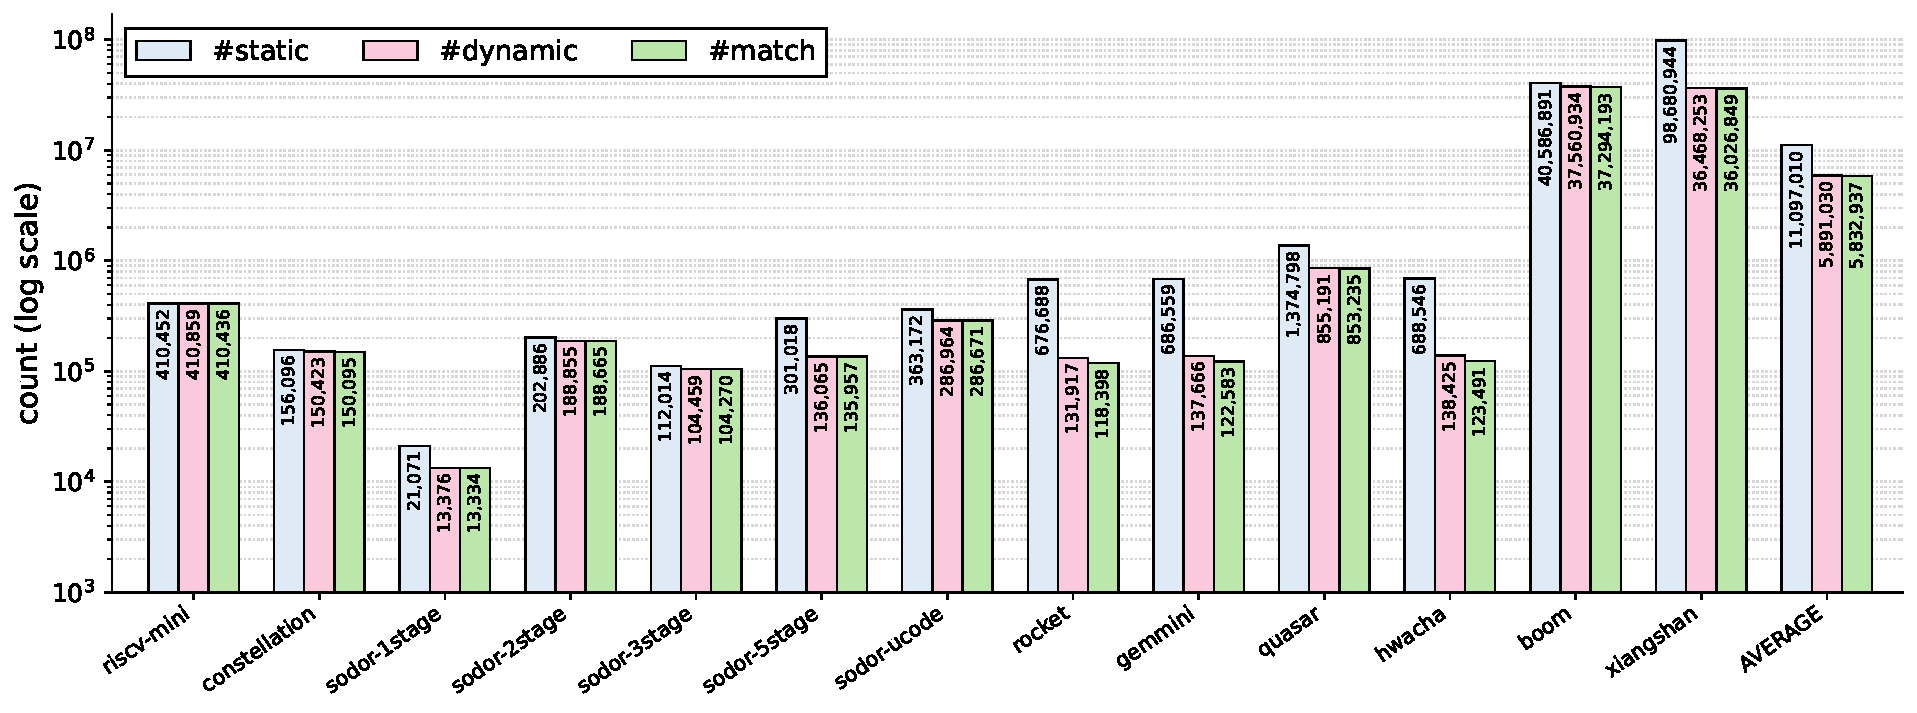
\includegraphics[width=\linewidth,clip,trim=8 10 15 12]{figures/tia-absolute-bars}
    \caption{\tia's results in revealing temporal influence relations in real-world Chisel designs.}\label{fig:tia-absolute}
\end{figure}


Figure~\ref{fig:tia-absolute} presents \tia's results in revealing temporal influence relations in real-world Chisel designs.
The absolute numbers of temporal influence relations captured by \tia (\texttt{\#static}), by runtime instrumentation (\texttt{\#dynamic}), and by both (\texttt{\#match}) are labeled on each bar.
The recall and precision calculated from the statistics in Figure~\ref{fig:tia-absolute} using Equation~\ref{eq:recall-precision} are presented in Figure~\ref{fig:tia-percent}.
Figure~\ref{fig:tia-percent} also presents the analysis time for each benchmark in the parentheses under the bars as an indication of \tia's efficiency.
Below, we separately detail \tia's soundness, precision, and efficiency based on these empirical results.

\begin{figure}[tp]
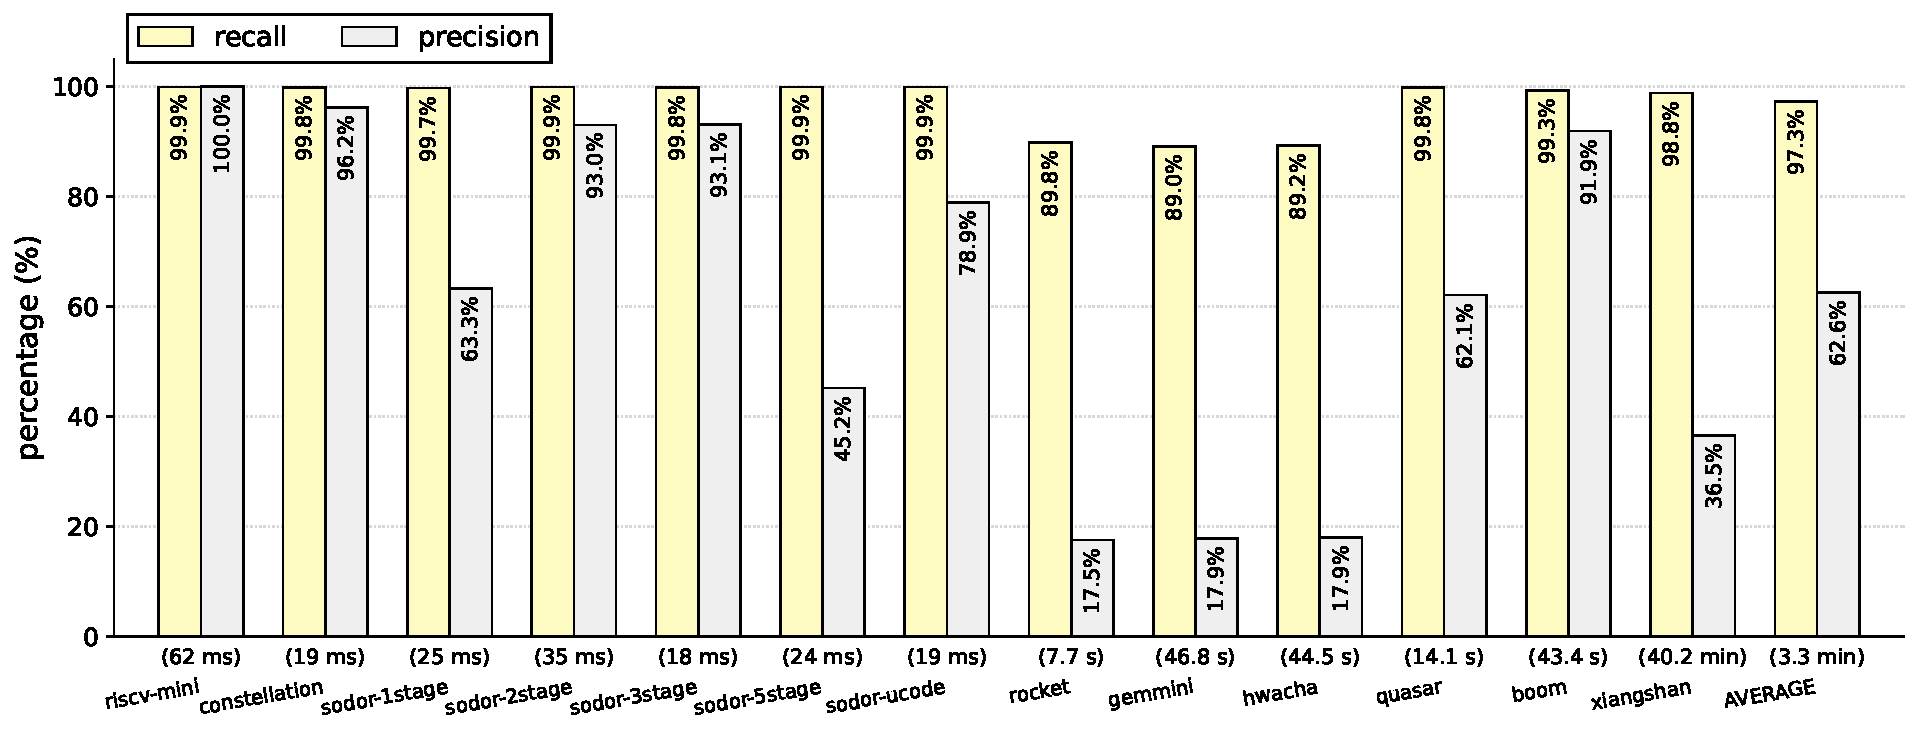
\includegraphics[width=\linewidth,clip,trim=8 9 18 5]{figures/tia-percent-bars}
\caption{Effectiveness of \tia on real-world Chisel designs, including recall (yellow bars), precision (gray bars), and efficiency (analysis time shown in parentheses under each bar).}\label{fig:tia-percent}
\end{figure}

\paragraph{Soundness}

\tia demonstrates strong empirical soundness, achieving an average recall of 97.3\%, as shown in the last column of Figure~\ref{fig:tia-percent}.
This high recall provides empirical evidence consistent with \tia's theoretical soundness. % TODO: in Theorems~\ref{theo:soundness} and~\ref{theo:}.
The small recall loss arises primarily from two limitations in handling complex real-world hardware designs.
(1) For external hardware modules whose source code is written in Verilog rather than Chisel, we model them as black boxes and assume a one-cycle delay between any input and output port.
This treatment is currently a heuristic engineering choice;
for example, the \texttt{plusarg\_reader} module in \texttt{rocket} cannot be soundly modeled using this heuristic.
Future work could investigate more systematic approaches, such as interactive static analysis across Chisel and Verilog.
(2) Since \tia's current theory focuses on synchronous hardware with a single global clock, for multiple-clock designs such as \texttt{hwacha} and \texttt{gemmini}, our implementation applies \tia rules independently to each clock domain as an engineering approximation.
This treatment may miss subtle temporal behaviors involving clock-domain crossings (CDCs)~\cite{chong_clock_2021}.
Future work could extend \tia's theory to multi-clock designs by explicitly tracking temporal influences with respect to each clock and developing rules for temporal interactions across clock domains.

\paragraph{Precision}
As the first static analysis primarily designed to soundly reason about infinite temporal influences in hardware designs, \tia achieves reasonable precision, with an average precision of 62.6\%, as shown in the last column of Figure~\ref{fig:tia-percent}.
This measured precision is an under-estimation of \tia's actual precision because we evaluate against only a subset of the true ground truth obtained through runtime instrumentation;
temporal influences reported by \tia but not observed dynamically may correspond to true influences that were simply not exercised during simulation.
Beyond this inherent under-estimation, we observe two major sources of imprecision in \tia.
\emph{(1) Memory Cell Insensitivity.}
For efficiency, we currently abstract an entire memory as a single abstract memory cell when analyzing memory accesses.
This coarse-grained abstraction can merge distinct temporal influence flows when they propagate through the memory, introducing false positives.
For example, the largest Chisel memory in \texttt{rocket} contains 16,384 cells, all of which are merged into a single abstract memory cell.
Although this abstraction is sound, it can introduce substantial imprecision.
A finer-grained memory abstraction could alleviate this problem and constitutes a direction for future work.
\emph{(2) Path Insensitivity.}
We currently soundly assume that the condition of each multiplexer (analogous to an \texttt{if}-statement in software) can evaluate to either true or false.
This path-insensitive treatment can introduce false positives.
For example, the conditions $a$ and $\neg a$ cannot both be true or both be false simultaneously, but our current analysis cannot exploit this mutual exclusivity to eliminate the corresponding false positives.
Introducing path sensitivity in the future could therefore further improve \tia's precision.


\paragraph{Efficiency}

As shown in Figure~\ref{fig:tia-percent}, \tia analyzes the 13 real-world hardware designs, totaling 5.9M LoC, in 42.8 minutes in total, 510.7$\times$ faster the 364.3 hours required by dynamic runtime instrumentation while achieving an average recall of 97.3\% in capturing dynamically observed temporal influences.
This result demonstrates the efficiency advantage of static analysis over simulation-based approaches for analyzing real-world hardware designs containing millions of lines of code.
The slowest case is \texttt{xiangshan}, which takes 40.2 minutes to analyze due to its large size of 4.0M LoC, yet remains substantially more efficient than dynamic simulation.


\subsection{RQ2: Potential of \tia to Support Diverse Hardware Analysis Clients}

To demonstrate the potential of \tia to support diverse hardware analysis clients, we develop three client analyses on top of \tia:
a hardware bug detection client---signal asynchrony analysis (Section~\ref{sec:client-asynchrony}),
a hardware security analysis client---timing-flow analysis (Section~\ref{sec:client-timingflow}),
and a hardware design understanding client---timeline interface analysis (Section~\ref{sec:client-timeline}).
We evaluate the three clients on their respective tasks to provide empirical evidence of \tia's practical potential.

\subsubsection{Hardware Bug Detection: Signal Asynchrony Analysis}\label{sec:eval-asynchrony}

The signal asynchrony analysis is described in Section~\ref{sec:client-asynchrony};
this section focuses on its evaluation (Figure~\ref{fig:eval-asynchrony}).

\begin{figure}[tp]
    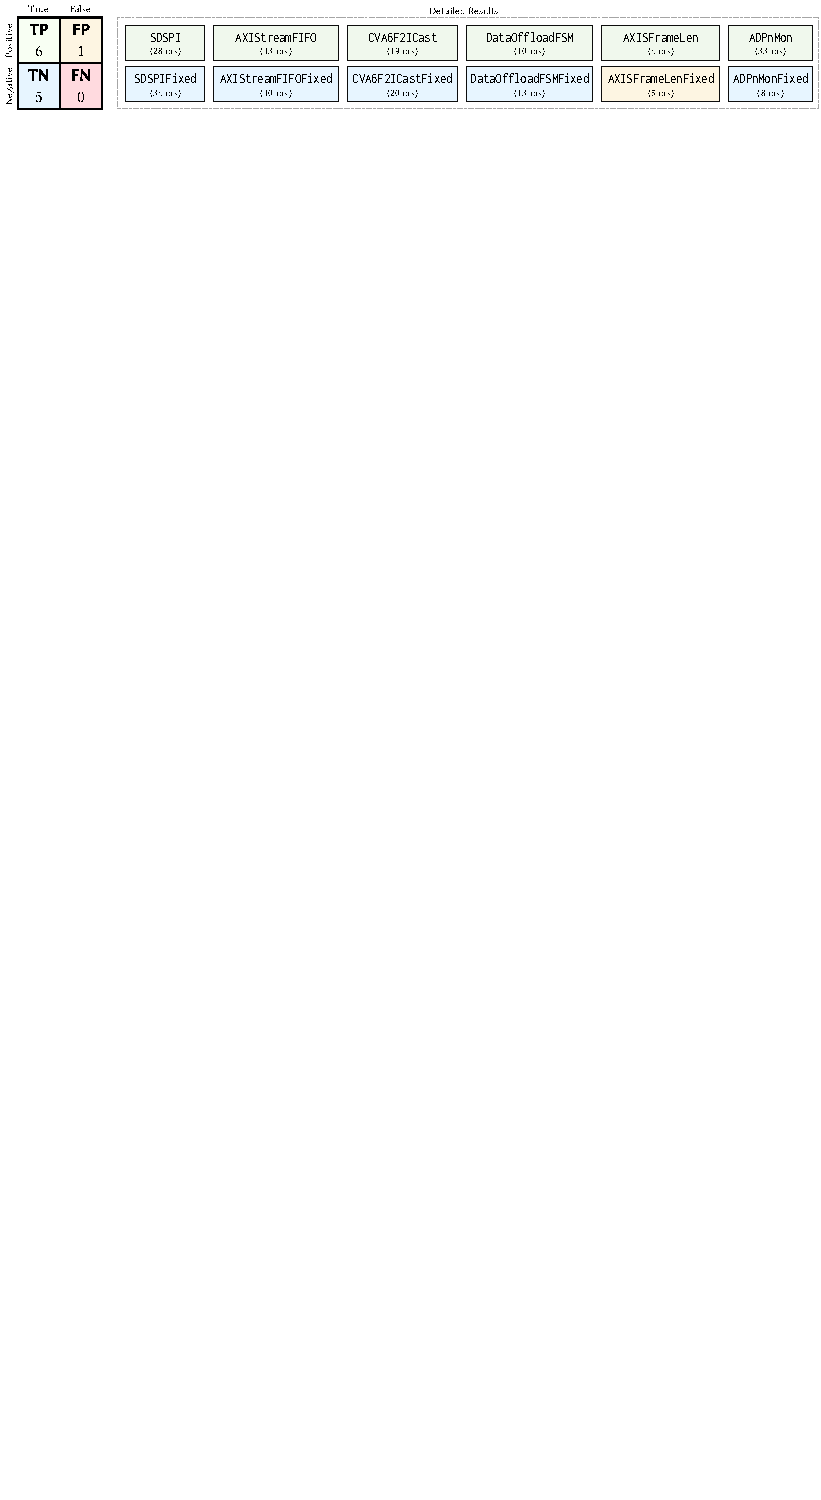
\includegraphics[clip,trim=0 23.5cm 0 0]{figures/asynchrony-eval}
    \caption{Evaluation of signal asynchrony analysis (recall: 100\%, precision: 85.7\%), a hardware bug detection client built on top of \tia; analysis times are shown in parentheses.}\label{fig:eval-asynchrony}
\end{figure}

\paragraph{Benchmarks}
Our signal asynchrony analysis is inspired by a survey of hardware bugs~\cite{ma_debugging_2022}, which defines signal asynchrony bugs and reproduces two such bugs from bug-fixing commits in open-source hardware projects: an SD card controller (\texttt{SDSPI}~\cite{sdspi}) and an AXI4-stream FIFO (\texttt{AXIStreamFIFO}~\cite{axi-stream-fifo}).
We use both the buggy and corresponding fixed versions of these two designs as benchmarks, yielding four benchmarks in the dashed box in Figure~\ref{fig:eval-asynchrony};
the fixed versions are denoted by appending the \texttt{Fixed} suffix to their original names.

The artifact~\cite{ma_debugging_2022_artifact} accompanying the survey~\cite{ma_debugging_2022} additionally lists eight signal asynchrony bug-fixing commits but does not provide proof-of-concept tests to reproduce their buggy behavior.
We attempted to reproduce these bugs and successfully developed proof-of-concept tests for four of them:
a floating-point unit (FPU) component (\texttt{CVA6F2ICast}~\cite{cva6-f2i-cast}),
a storage unit access controller (\texttt{DaraOffloadFSM}~\cite{data-offload-fsm}),
a network interface controller component for frame monitoring (\texttt{AXISFrameLen}~\cite{axis-frame-len}), and
a pseudo-random number monitor (\texttt{ADPnMon}~\cite{ad-pn-mon}).
Together with their corresponding fixed versions, these four buggy designs yield eight additional benchmarks, also shown in the dashed box in Figure~\ref{fig:eval-asynchrony}.

For the remaining four bug-fixing commits listed in the artifact~\cite{ma_debugging_2022_artifact}, our investigation found that three are outside the scope of the signal asynchrony bugs defined by the survey.
The remaining commit modifies 68 files, and we could not identify a reproducible signal asynchrony bug from it.

\paragraph{Understanding the Results}
The left part of Figure~\ref{fig:eval-asynchrony} summarizes the overall results of signal asynchrony analysis, while the right part details the results for each benchmark, with colors indicating the classification.
There are 6 true positives (TPs, in green), where our analysis correctly identifies buggy designs as buggy, and 5 true negatives (TNs, in blue), where it correctly identifies non-buggy designs as non-buggy.
There are no false negatives (FNs, in red), where our analysis fails to detect a true asynchrony bug, yielding a recall of $\mathit{recall} = \mathit{TP}/(\mathit{TP}+\mathit{FN}) = 100\%$.
There is only one false positive (FP, in yellow), where our analysis reports a asynchrony bug in a non-buggy design, yielding a precision of $\mathit{precision} = \mathit{TP}/(\mathit{TP}+\mathit{FP}) = 85.7\%$.

The false positive occurs in \texttt{AXISFrameLenFixed}.
This module expects its AXI monitor interface inputs to follow a specific protocol, under which its outputs \texttt{frameLen} and \texttt{frameLenValid} are synchronized by the input \texttt{monitorAxisTlast}.
However, our analysis does not incorporate this input constraint and therefore considers these outputs potentially asynchronous under unconstrained inputs.
Thus, although the bug is fixed under the module's intended input protocol, our analysis reports a potential asynchrony under unconstrained inputs, resulting in the false positive.

As indicated by the analysis times in parentheses under the benchmark names in Figure~\ref{fig:eval-asynchrony}, our signal asynchrony analysis is also efficient, taking an average of 16.4 milliseconds across the benchmarks, including the time spent by the underlying \tia.
This efficiency stems from both the efficiency of \tia and the lightweight reuse of its computed temporal influence information: the client analysis only queries \tia's results to check signal synchronization, as described in Section~\ref{sec:client-asynchrony}, and therefore incurs little additional computational overhead.

\subsubsection{Hardware Security Analysis: Timing-flow Analysis}

The timing-flow analysis is described in Section~\ref{sec:client-timingflow};
this section focuses on its evaluation (Figure~\ref{fig:eval-timingflow}).

\begin{figure}[tp]
    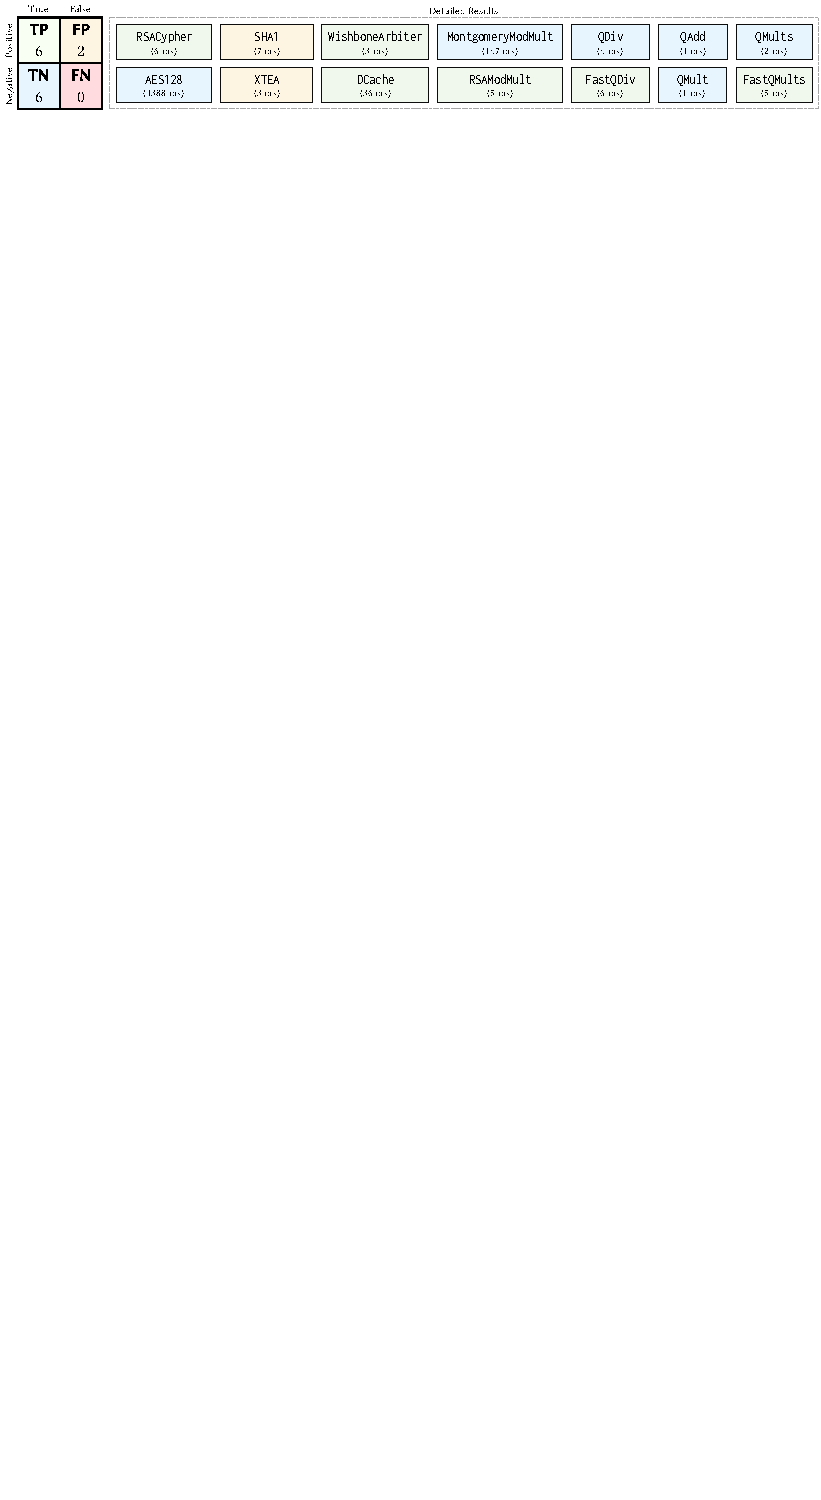
\includegraphics[clip,trim=0 23.5cm 0 0]{figures/timingflow-eval}
    \caption{Evaluation of timing-flow analysis (recall: 100\%, precision: 75\%), a hardware security client built on top of \tia; analysis times are shown in parentheses.}\label{fig:eval-timingflow}
\end{figure}

\paragraph{Benchmarks}

Our timing-flow analysis is inspired by a survey of hardware information-flow tracking~\cite{hu_hardware_2022}, which describes information leaks through timing flows and summarizes representative hardware designs for which prior work~\cite{ardeshiricham_clepsydra_2017,qin_formal_2020,alatoun_efficient_2022} has established the presence or absence of timing flows.
We select all such designs available to us as benchmarks to evaluate our timing-flow analysis.
These designs, shown in the dashed box in the right part of Figure~\ref{fig:eval-timingflow}, include cryptographic components from TrustHub~\cite{salmani_design_2013,shakya_benchmarking_2017} (\texttt{RSACypher}~\cite{rsa-cypher} and \texttt{AES128}~\cite{aes128}) and OpenCores~\cite{opencores} (\texttt{SHA1}~\cite{sha1} and \texttt{XTEA}~\cite{xtea}), a round-robin-based Wishbone arbiter (\texttt{WishboneArbiter}~\cite{wishbone-arbiter}), a data cache (\texttt{DCache} described by~\cite{qin_formal_2020}), modular multipliers (\texttt{MontgomeryModMult}~\cite{montgomery-modmult} and \texttt{RSAModMult}~\cite{rsa-modmult}), and fixed-point arithmetic units~\cite{fixed-point-math} and their variants described by~\cite{qin_formal_2020,ardeshiricham_clepsydra_2017}.

\paragraph{Understanding the Results}


The left part of Figure~\ref{fig:eval-timingflow} summarizes the overall results of timing-flow analysis, while the right part details the results for each benchmark, with colors indicating the classification.
There are 6 true positives (TPs, in green), where our analysis correctly identifies timing-flow information leaks in vulnerable designs, and 6 true negatives (TNs, in blue), where it correctly identifies secure designs without timing flows as secure.
There are no false negatives (FNs, in red), where our analysis fails to detect a true timing-flow information leak, yielding a recall of $\mathit{recall} = \mathit{TP}/(\mathit{TP}+\mathit{FN}) = 100\%$.
There are two false positives (FPs, in yellow), where our analysis reports a timing-flow information leak in a secure design, yielding a precision of $\mathit{precision} = \mathit{TP}/(\mathit{TP}+\mathit{FP}) = 75\%$.
The two false positives occur in \texttt{SHA1} and \texttt{XTEA} and are caused by \tia's path insensitivity.
Specifically, path insensitivity allows spurious temporal influences from the private source to the public sink that indicate timing flows, even though not all of these influences can occur under the actual combination of multiplexer conditions.

As indicated by the analysis times in parentheses under the benchmark names in Figure~\ref{fig:eval-timingflow}, our timing-flow analysis is also efficient, taking an average analysis time of 115.3 milliseconds across the benchmarks, including the time spent by the underlying \tia.
This efficiency stems from both the efficiency of \tia and the lightweight reuse of its computed temporal influence information: the client analysis only queries \tia's results to identify multiple temporal influences that indicate timing flows, as described in Section~\ref{sec:client-timingflow}, and therefore incurs little additional computational overhead.
The \texttt{AES128} benchmark takes more than one second to analyze, substantially longer than the other benchmarks combined, because it is much larger than the other benchmarks combined (98.4K LoC vs. 1.6K LoC in pre-elaborated Firrtl~\cite{izraelevitz_reusability_2017}).

\subsubsection{Hardware Design Understanding: Timeline Interface Analysis}

The timeline interface analysis is described in Section~\ref{sec:client-timeline};
this section focuses on its evaluation (Figure~\ref{fig:eval-timeline}).

\begin{figure}[tp]
    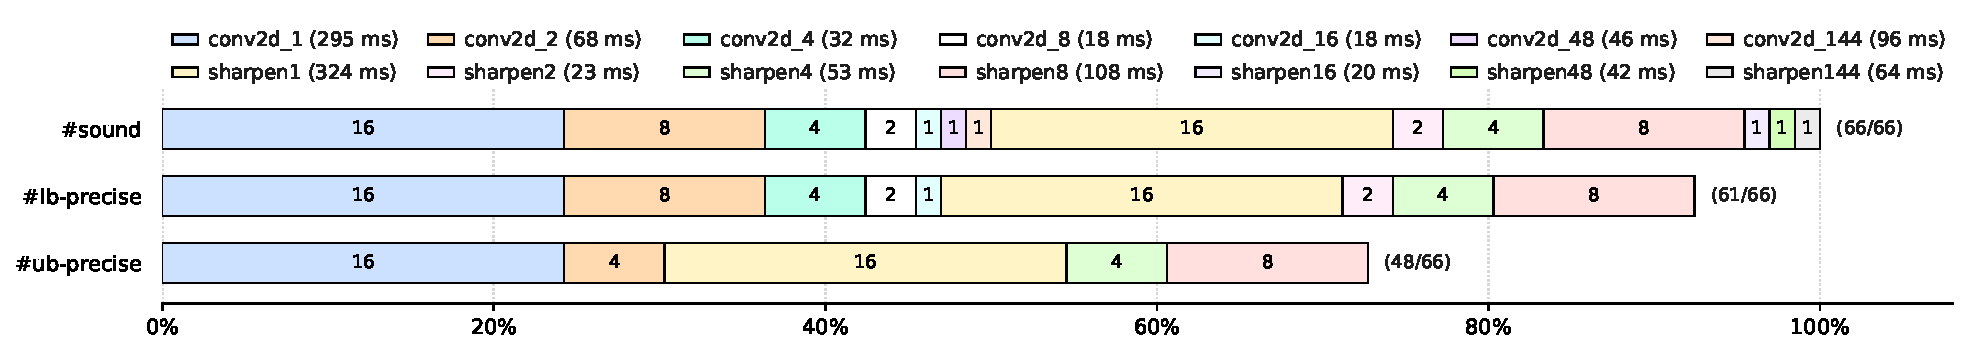
\includegraphics[width=\linewidth,clip,trim=8 9 11 15]{figures/timeline-eval}
    \caption{
        Evaluation of timeline interface analysis (a hardware design understanding client built on top of \tia), where \texttt{\#sound} denotes the number of inferred timeline intervals that are supersets of the corresponding ground-truth intervals (recall: 100\%),
        \texttt{\#lb-precise} denotes the number of inferred timeline intervals with a precise lower bound (lower-bound precision: 92.4\%), and
        \texttt{\#up-precise} denotes the number of inferred intervals with a precise upper bound (upper-bound precision: 72.7\%).
        Analysis times are shown in parentheses.
    }\label{fig:eval-timeline}
\end{figure}

\paragraph{Benchmarks}

Our timeline interface analysis is inspired by the hardware timeline type system~\cite{nigam_modular_2023}, which specifies the clock-cycle intervals during which each input or output is required or available, providing a convenient interface for hardware designers to understand the temporal behavior of a hardware module.
We therefore reuse the hardware designs evaluated in~\cite{nigam_modular_2023}, whose timeline interfaces are established by the type system, as benchmarks for evaluating our timeline interface analysis.
The benchmarks include 14 designs, shown in Figure~\ref{fig:eval-timeline}, implementing two image-processing accelerator kernels (\texttt{conv2d} and \texttt{sharpen}), with 7 design points for each kernel representing different resource-throughput trade-offs.

\paragraph{Understanding the Results}

Figure~\ref{fig:eval-timeline} presents the results of timeline interface analysis.
Across the 66 top-module output ports in the benchmarks, our timeline interface analysis infers 66 timeline intervals with the following results.
\emph{First}, all 66 inferred intervals are sound, i.e., they are supersets of the corresponding ground-truth intervals, yielding a recall of 100\%.
\emph{Second}, 61 inferred intervals have a precise lower bound, yielding a lower-bound precision of $61/66 = 92.4\%$.
\emph{Third}, 48 inferred intervals have a precise upper bound, yielding an upper-bound precision of $48/66 = 72.7\%$.
Thus, the upper-bound precision is lower than the lower-bound precision.

The lower upper-bound precision is primarily caused by imprecision in the underlying \tia, which can introduce false-positive temporal influences at larger, potentially unbounded clock cycles due to widening and path insensitivity.
For example, in \texttt{conv2d\_4}, each output has a ground-truth timeline interval of $[G+6, G+7)$, whereas our timeline interface analysis reports $[G+6, G+9)$.
Although the inferred interval is sound and has a precise lower bound, its upper bound is imprecise because the underlying \tia reports two false-positive temporal influence objects at clock cycles 7 and 8.
In the worst case, the inferred upper bound is infinity, which occurs for 4 of the 66 ports.
For example, the output port $O$ of \texttt{conv2d\_48} has a ground-truth timeline interval of $[G+12, G+13)$, whereas our analysis reports $[G+9, G+\infty)$.
This imprecision arises because path insensitivity in the underlying \tia can introduce a loop in the temporal influence graph (TIG), causing infinitely many temporal influences to propagate to $O$ and resulting in an infinite upper bound, as described in Section~\ref{sec:client-timeline}.
We think improving the precision of \tia in future work could improve the precision of this hardware design understanding client.

As indicated by the analysis times in parentheses to the right of the benchmark names in Figure~\ref{fig:eval-timeline}, our timeline interface analysis is efficient, taking an average analysis time of 86.2 milliseconds across the benchmarks, including the time spent by the underlying \tia.
This efficiency stems from both the efficiency of \tia and the lightweight reuse of its computed temporal influence information: the client analysis only queries \tia's results to compute the minimal interval containing all clock cycles occurring in the temporal influence objects, as described in Section~\ref{sec:client-timeline}, and therefore incurs little additional computational overhead.




